%%%%%%%%%%%%%%%%%%%%%%%%%%%%%%%%%%%%%%%%%%%%%%%%%%%%%%%%%%%%%%%%%%%%
%%
%%                     Resultados
%%
%%%%%%%%%%%%%%%%%%%%%%%%%%%%%%%%%%%%%%%%%%%%%%%%%%%%%%%%%%%%%%%%%%%%

\begin{frame}{Deteção da barra}
   \begin{figure}[H]
    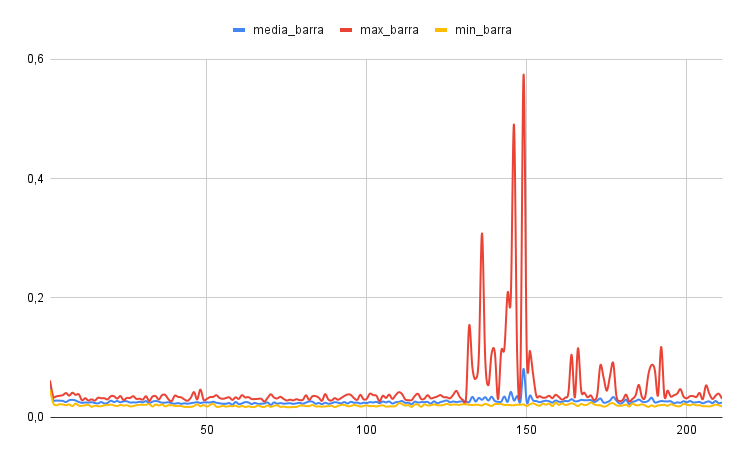
\includegraphics[width=11cm]{img/resultados/barra.png}
    {Fonte: Próprio Autor}
    \label{figura:configs_server}
    \end{figure}
\end{frame}

\begin{frame}{Inclinação da barra}
   \begin{figure}[H]
    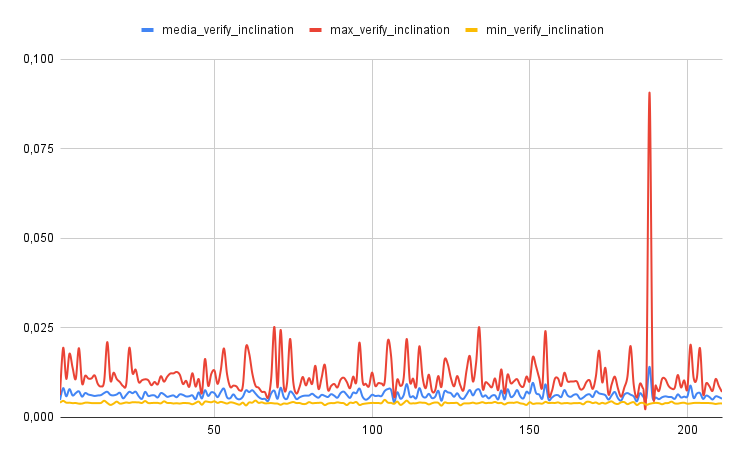
\includegraphics[width=11cm]{img/resultados/inclination.png}
    {Fonte: Próprio Autor}
    \label{figura:configs_server}
    \end{figure}
\end{frame}

\begin{frame}{Estimativa de pose humana}
   \begin{figure}[H]
    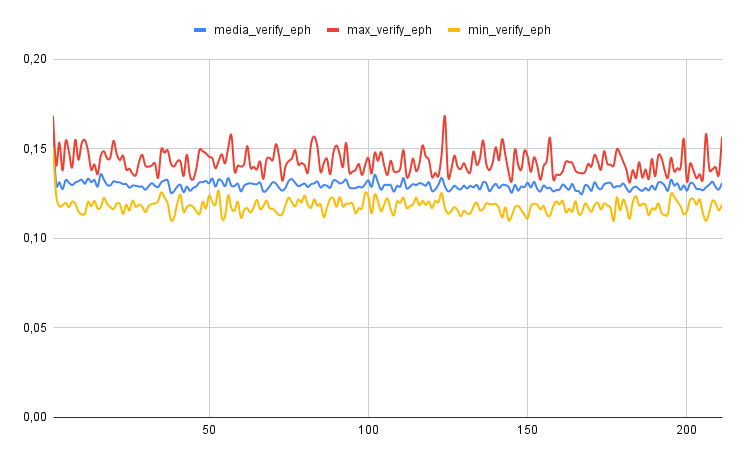
\includegraphics[width=11cm]{img/resultados/eph.png}
    {Fonte: Próprio Autor}
    \label{figura:configs_server}
    \end{figure}
\end{frame}

\begin{frame}{Construção do caracter do AFD}
   \begin{figure}[H]
    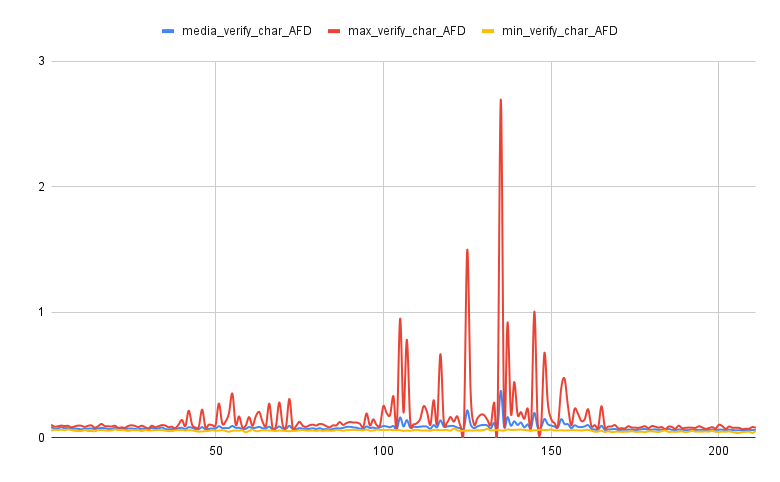
\includegraphics[width=11cm]{img/resultados/char_AFD.png}
    {Fonte: Próprio Autor}
    \label{figura:configs_server}
    \end{figure}
\end{frame}

\begin{frame}{Composição das funções que formam o caracter }
   \begin{figure}[H]
    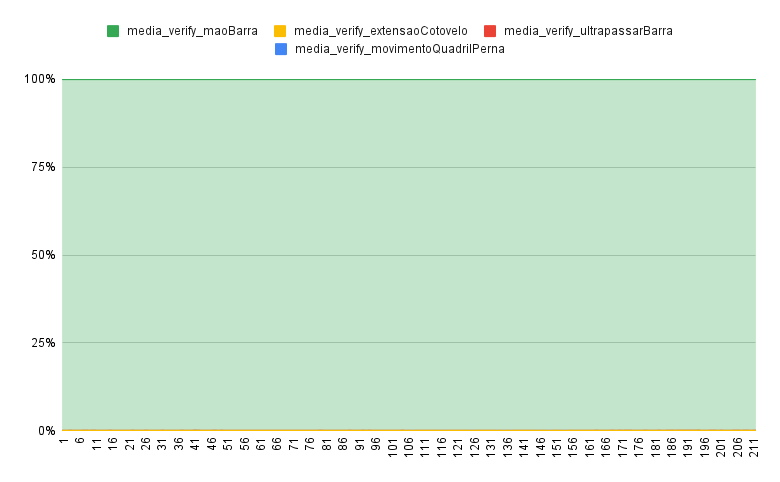
\includegraphics[width=11cm]{img/resultados/comp_char_AFD.png}
    {Fonte: Próprio Autor}
    \label{figura:configs_server}
    \end{figure}
\end{frame}

\begin{frame}{Mão na barra}
   \begin{figure}[H]
    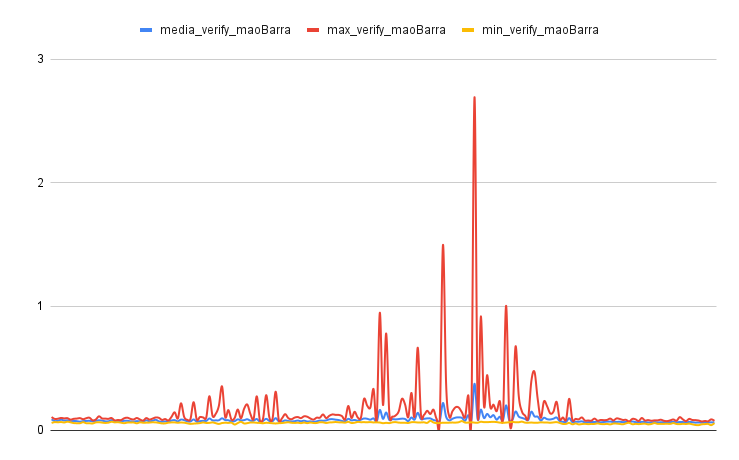
\includegraphics[width=11cm]{img/resultados/maoBarra.png}
    {Fonte: Próprio Autor}
    \label{figura:configs_server}
    \end{figure}
\end{frame}

\begin{frame}{Braço extendido}
   \begin{figure}[H]
    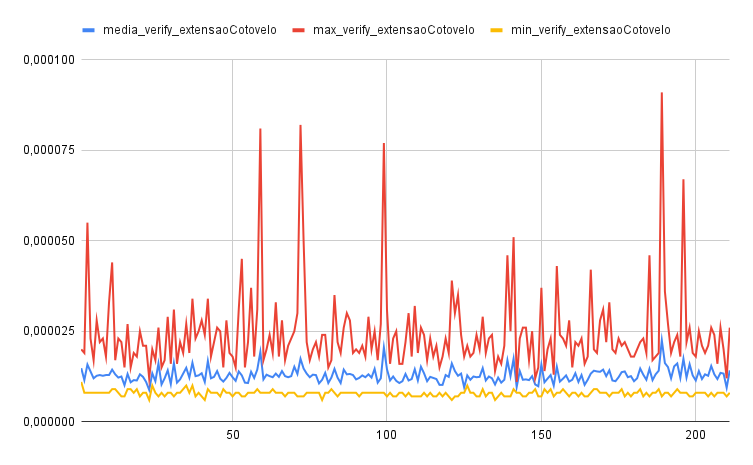
\includegraphics[width=11cm]{img/resultados/extensaoCotovelo.png}
    {Fonte: Próprio Autor}
    \label{figura:configs_server}
    \end{figure}
\end{frame}

\begin{frame}{Ultrapassar o queixo á barra}
   \begin{figure}[H]
    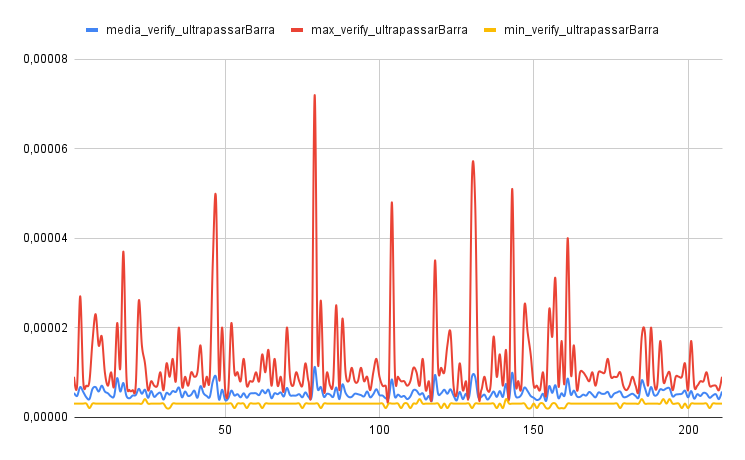
\includegraphics[width=11cm]{img/resultados/ultrapassarBarra.png}
    {Fonte: Próprio Autor}
    \label{figura:configs_server}
    \end{figure}
\end{frame}

\begin{frame}{Movimento das pernas e do quadril}
   \begin{figure}[H]
    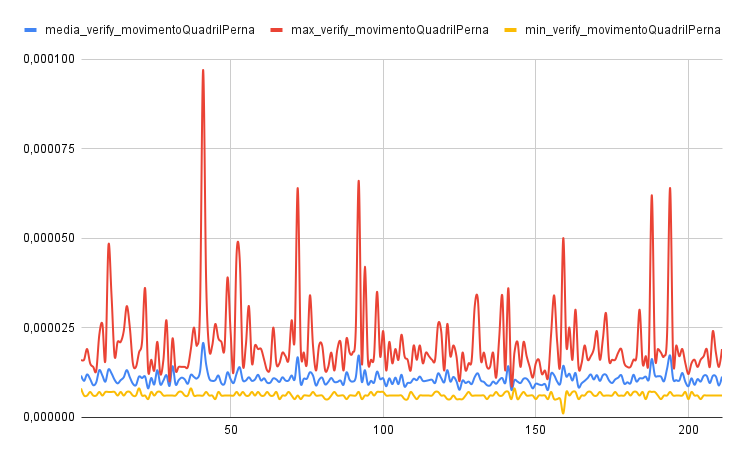
\includegraphics[width=11cm]{img/resultados/movimentoQuadril.png}
    {Fonte: Próprio Autor}
    \label{figura:configs_server}
    \end{figure}
\end{frame}




\begin{frame}{Processamento de um frame}
   \begin{figure}[H]
    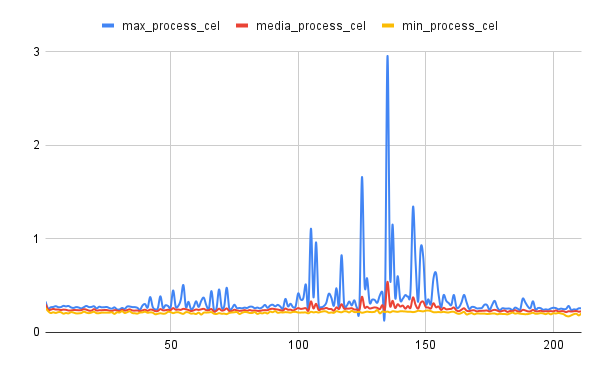
\includegraphics[width=11cm]{img/resultados/process_cell.png}
    {Fonte: Próprio Autor}
    \label{figura:configs_server}
    \end{figure}
\end{frame}


\begin{frame}{Composição das funções necessárias para processar um frame}
   \begin{figure}[H]
    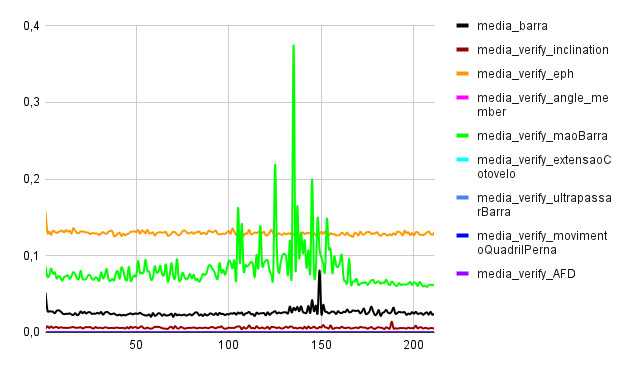
\includegraphics[width=11cm]{img/resultados/comp_process_cell_2.png}
    {Fonte: Próprio Autor}
    \label{figura:configs_server}
    \end{figure}
\end{frame}


\begin{frame}{Composição das funções necessárias para processar um frame}
   \begin{figure}[H]
    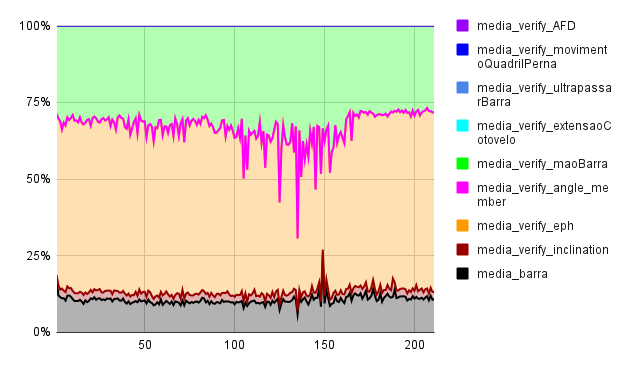
\includegraphics[width=11cm]{img/resultados/comp_process_cell_1.png}
    {Fonte: Próprio Autor}
    \label{figura:configs_server}
    \end{figure}
\end{frame}


%%%%%%%%%%%%%%%%%%%%%%%%%%%%%%%%%%%%%%%%%%%%%%%%%%%%%%%%%%%%%%%%%%%%
%%
%%                     Mensuração
%%
%%%%%%%%%%%%%%%%%%%%%%%%%%%%%%%%%%%%%%%%%%%%%%%%%%%%%%%%%%%%%%%%%%%%



\begin{frame}{Resultados Experimentos}
    \fontsize{7pt}{8pt}\selectfont
    \begin{table}[H]
    \centering
    \begin{tabular}{@{}cccccc@{}}
    \toprule
    \multicolumn{6}{c}{Tempos médios e menores tempos registrados para cada função}
    \\ \midrule
    Função & Tempo médio (s) & Menor tempo(s) \\
    \midrule
    barra & 0,03422 & 0,016335 \\
    verify\_inclination & 0,00603 & 0,00317 \\
    verify\_eph & 0,1293617 & 0,109623 \\
    verify\_angle\_member & 0,00013 & 0,000045 \\
    verify\_char\_AFD & 0,0753571 & 0,039386 \\
    verify\_AFD & 0,0000427 & 0,000016 \\
    \bottomrule
    \end{tabular}
    \label{tab:tempos_funcoes}
    \\
    {Fonte: Próprio Autor}
    \end{table}
\end{frame}






\begin{frame}{Resultados Experimentos}
    \fontsize{7pt}{8pt}\selectfont
    \begin{table}[H]
    \centering
    \begin{tabular}{@{}cccccc@{}}
    \toprule
    \\ \midrule
    Função & Tempo médio (s) & Menor tempo (s) \\
    \midrule
    verify\_maoBarra & 0,0747025 & 0,03924 \\
    verify\_extensaoCotovelo & 0,0000126 & 0,000006  \\
    verify\_ultrapassarBarra & 0,0000051 & 0,000002  \\
    verify\_movimentoQuadrilPerna & 0,0000104 & 0,000001  \\
    \bottomrule
    \end{tabular}
    \label{tab:tempos_funcoes_especificas}
    \\
    {Fonte: Próprio Autor}
    \end{table}
\end{frame}
